\section{System performances}

\subsection{Test system}
All the machine used for testing purposes are Openstack virtual machines, with
the following specifications:
\begin{itemize}
\item 1 machine with 32GB of RAM, 8vCPU and solid state storage. This host was
used as final destination of packets;
\item 4 machines with 16GB of RAM, 6vCPU and solid state storage. These VMs
were utilized to form the Kubernetes cluster, on the top of which the SFC
infrastructure developed was running;
\item 1 machine with 4GB of RAM, 2vCPU and solid state storage. This host on
was used as client and on which run script to send packets.
\end{itemize}

\subsection{RTT measurement}
Regarding the delivery performance, a metric to take in account is the
\emph{round trip time}(RTT), that is the time interval between the instant in
which a packet is sent and when the response is received. To analyze it we
developed a Python script that sends a packet (with 8B of payload) and waits for
the correspondent response, recording the instants (expressed as \emph{epoch})
of transmission and receiving. The goal of this test is to compare the average
RTT measured without involving any SFC (therefore simply delivering the packet
to the receiver and get back the reply) with the RTT in the case in which
packets pass through different length SFCs. In particular, this experiments was
repeated with chains that have 1, 2, 3, 4, 5, and 10 hops respectively. It is
useful to remember that packets traverse the SFC on both sides: SF that are
used only prints the packet received and the total number of packets that have
passed through it. Results are collected after 100 repetitions of the test.

\begin{table}[H]
\centering
\begin{tabular}{@{}cc@{}}
\toprule
\textbf{SFC length} & \textbf{Mean RTT (Seconds)} \\ \midrule
len. 0              & 0.0009668279      \\
len. 1              & 0.0555884027      \\
len. 2              & 0.0702438903      \\
len. 3              & 0.0888472247      \\
len. 4              & 0.1045638967      \\
len. 5              & 0.1239343858      \\
len. 10             & 0.2135494161      \\ \bottomrule
\end{tabular}
\caption{Mean RTT measured with different SFC length}
\label{chap:tests:sec:rtt:tab:meanrtt}
\end{table}

Not surprisingly, as depicted in the Table~\ref{chap:tests:sec:rtt:tab:meanrtt},
the RTT is bigger when packets travel through the chain and it increases with
the total number of elements of the SFC. There is a large
difference between the mean RTT of the configuration without any chain and the
one with an SFC with a single link: this outcome has different explanation. As
described in \todo{Add reference to implementation} the chain has always at
least 3 hops (ingress, SF, egress), so the packet must be elaborated by 3
different running software. Another interpretation lays into how the code was
written: components of these framework are not developed as a production ready
software, but for a proof of concept, so connections and transmissions can be
enhanced. Finally, SFs are meant to perform some modifications to the packet,
so, unavoidably, some time is required for their computation.

\begin{figure}[H]
  %\centering
    \begin{subfigure}[b]{0.45\textwidth}
        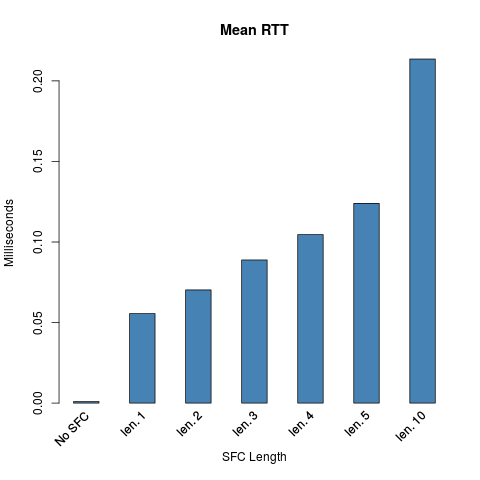
\includegraphics[scale=0.4]{meanrtt}
        \caption{Mean RTT calculate using SFCs of different lengths}
        \label{chap:tests:sec:rtt:img:meanstt}
    \end{subfigure}
    ~
    \begin{subfigure}[b]{0.45\textwidth}
        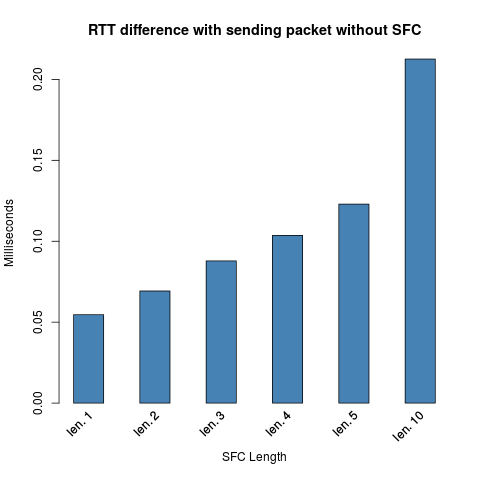
\includegraphics[scale=0.4]{differencenosfc}
        \caption{Time increase using SFCs of different lengths}
        \label{chap:tests:sec:rtt:img:differencertt}
    \end{subfigure}
\end{figure}

The results on average RTT are better represented in
Figure~\ref{chap:tests:sec:rtt:img:meanstt}. In that graph we can easily see
the difference among the different configurations. Looking at the bars in the
center, representing the SFCs composed by 1, 2, 3, 4 and 5 links, we can see a
fairly linear increase of the RTT. This trend strongly depends on the nature of
the SF involved in the chain, and in this experiment the linear increase is
highlighted due to the usage of the same function for each hop. In
Figure~\ref{chap:tests:sec:rtt:img:differencertt} we can see the additional
time required for each transmission with the different SFCs, calculated as the
difference between the average RTT of a specific chain and the RTT measured
without involving any SFC. Event in that plot we can see a quite linear
increase depending on the length of the chain.

\begin{figure}[H]
  \centering
  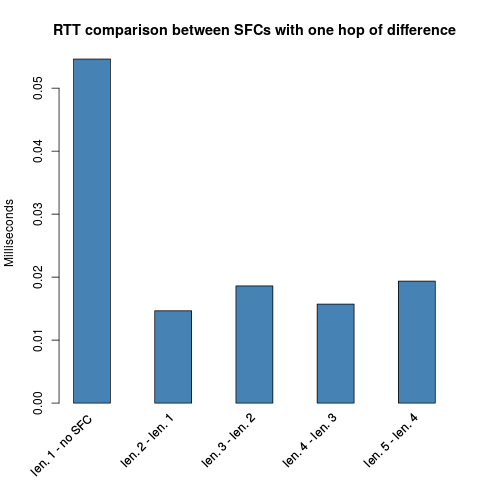
\includegraphics[scale=0.4]{differenceonehop}
  \caption{Time difference between SFCs that have a length difference of one SF}
  \label{chap:tests:sec:rtt:img:differenceonehop}
\end{figure}

In Figure~\ref{chap:tests:sec:rtt:img:differenceonehop} is represented the
difference in terms of average RTT between chains whose lengths differs only by
one link. The highest value was calculated bringing into comparison the direct
deliver of packets and the chain of only one element: even in that case is
remarked that SFC cost time in the context of transmission of single packets.
Other differences among SFC, instead, are quite similar, highlighting the
linear trend.

\begin{table}[H]
\centering
\begin{tabular}{@{}cc@{}}
\toprule
\textbf{SFC Length} & \textbf{Jitter(Seconds)} \\ \midrule
len. 0    & 0.0001484817    \\
len. 1    & 0.0034793676    \\
len. 2    & 0.0040213103    \\
len. 3    & 0.0036568939    \\
len. 4    & 0.0031962546    \\
len. 5    & 0.0046836929    \\
len. 10   & 0.0073287308    \\ \bottomrule
\end{tabular}
\caption{Jitter for different SFC lengths}
\label{chap:tests:sec:rtt:tab:jitter}
\end{table}

Another metric to take in account is jitter. Jitter is the variation in the
delay of received packet, and gives a measure of the congestion of the network
or underline other communication problems.
Table~\ref{chap:tests:sec:rtt:tab:jitter} represent the jitter calculated for
different SFC length, derived from values of RTT measured in the previous test.
As we can see values are really low, indicating no particular problems on the
network, even if the lowest result is always the one calculated without the
chain.

\subsection{Resilience}
Regarding the overall system resilience, we performed some test in which some
nodes of our solution are stopped during a transmission. As a matter of fact
that one of the most important requirements of our implementation is to make
the system  able to recover after an SF crash. Exploiting Docker container
technology and Kubernetes platform it is quite straightforward to restart a
container after a fault. In fact, \texttt{yaml} files that allows to deploy
containers on Kubernetes, make possible to set pods restart policy to
``always'' (the default one), ``on failure'' or ``never'', but the overall
system must be able to recognize that the SF is brought up again. 

During this test test we forward 500 packets (1 packet each 50ms) from a sender
host to a receiver through an SFC of length 3. The \texttt{yaml} file
describing the chain is the following:

\lstinputlisting[caption={Kubernetes YAML configuration that has been used for
resilience test}, captionpos=b]{res/code/fault_test.yaml}

The previous configuration can be represented as in
Figure~\ref{chap:tests:sec:fault:img:testfaultconf}.
\begin{figure}[H]
  \centering
  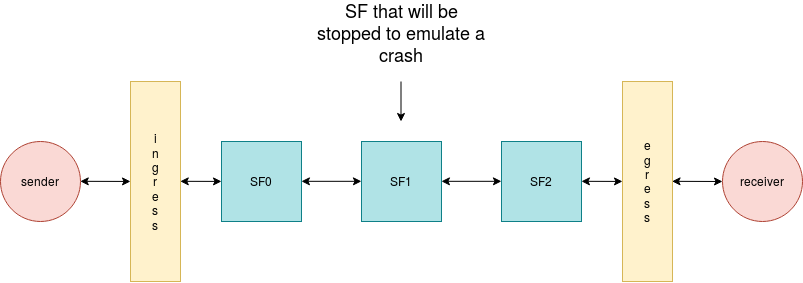
\includegraphics[scale=0.4]{testfaultconf}
  \caption{Host logical configuration for testing}
  \label{chap:tests:sec:fault:img:testfaultconf}
\end{figure}

In that test we bring down the central link of the chain after 5 seconds using
the command \verb!kubectl delete pods <pod-id> --grace-period=0 --force!, to
force the stop of a pod and we recorded the time on which packets arrived to
the receiver and passed through the VNF just before the one that will be make
stopped.

We performed the test using both UDP and TCP protocols, repeating for each
protocol the measurement 20 times.
Figure~\ref{chap:tests:sec:fault:img:faultgraphudp} and
Figure~\ref{chap:tests:sec:fault:img:faultgraphtcp} represent the behavior of
the system during the experiment: blue points describe packet inter-arrival
time on the receiver, green once the same metric on the SF that precede the
central one. The average interval of time in which the
receiver does not receive anything was 13.5793391228s in case of UDP,
13.7828050137s in case of TCP. This is a good result, because in about 13s a
machine can crash and can be recreated and be operative again. 

\begin{figure}[]
  %\centering
    \begin{subfigure}[b]{0.9\textwidth}
        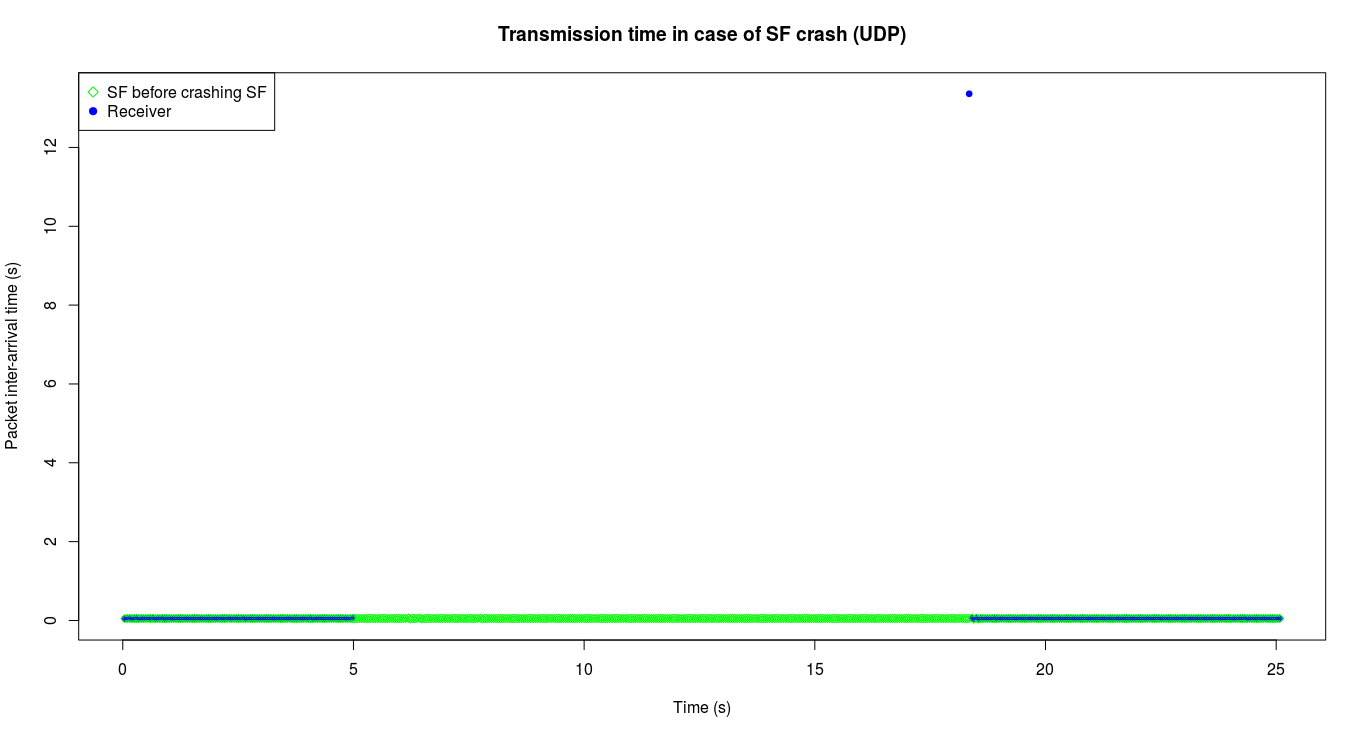
\includegraphics[scale=0.3]{udp_fault}
        \caption{Packet time arrival in case of SF fault using UDP}
        \label{chap:tests:sec:fault:img:faultgraphudp}
    \end{subfigure}
    \\
    \begin{subfigure}[b]{0.9\textwidth}
        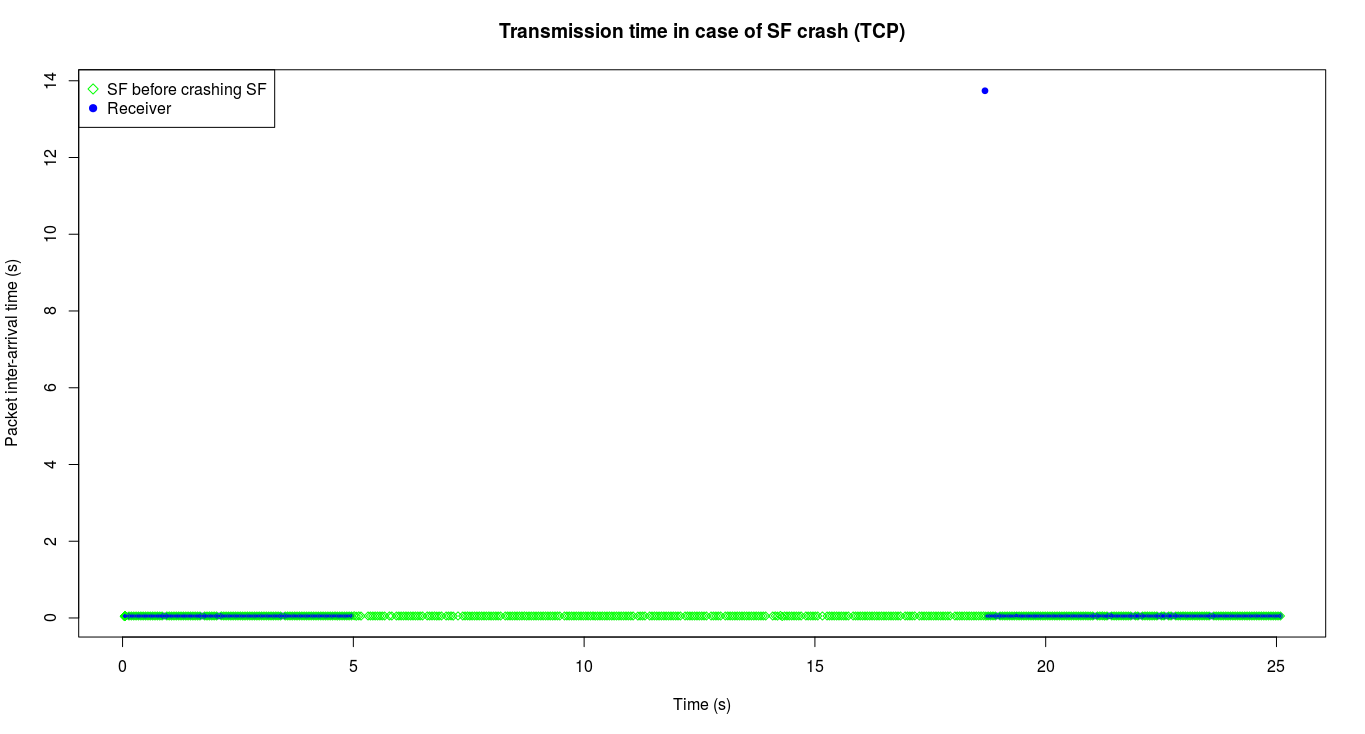
\includegraphics[scale=0.3]{tcp_fault}
        \caption{Packet time arrival in case of SF fault using TCP}
        \label{chap:tests:sec:fault:img:faultgraphtcp}
    \end{subfigure}
    \caption{Comparison among TCP and UDP in terms of packet time arrival in
    case of SF fault}
    \label{chap:tests:sec:fault:img:faultgrapht}
\end{figure}

After those results, we repeated the test (this time only using UDP) with the
configuration and shown in
Figure~\ref{chap:tests:sec:fault:img:testfaultconfwithreplica}, in order to
test the resilience of the system in case of a replica of a certain SF. We
repeated this experiment 10 times, bringing down only one of the 2 replica of
the same SF and we were not able to record any significant interval of time in
which the receiver does not received packet (receiving times are consistent
with sending times). So we can consider that in case of light traffic only 2
replicas of a specific function can be enough to offer to final user a reliable
service.

\begin{figure}[H]
  \centering
  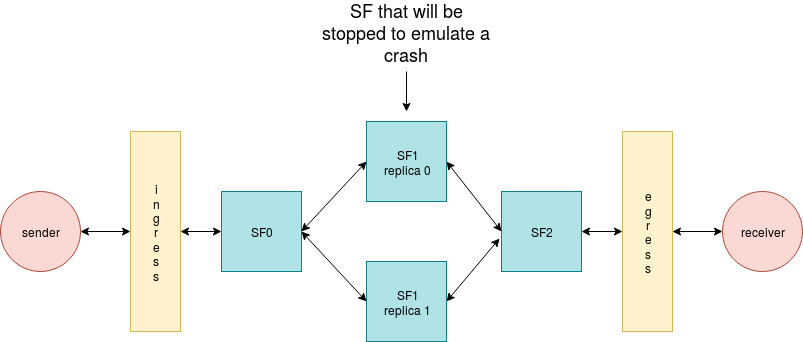
\includegraphics[scale=0.4]{testfaultconfwithreplica}
  \caption{Host logical configuration in case of a replicated SF for testing}
  \label{chap:tests:sec:fault:img:testfaultconfwithreplica}
\end{figure}